\documentclass[12pt,a4paper]{article}
\usepackage[T2A]{fontenc}
\usepackage[utf8]{inputenc}
\usepackage[russian]{babel}
\usepackage{amsmath,amssymb,amsthm}
\usepackage{geometry}
\usepackage{hyperref}
\usepackage{microtype}
\usepackage{setspace}
\usepackage{caption}
\usepackage{graphicx}

\geometry{left=25mm, right=25mm, top=25mm, bottom=25mm}

\hypersetup{
  colorlinks=true,
  linkcolor=black,
  urlcolor=blue,
  pdfauthor={Тишковец Сергей},
  pdftitle={Отчёт по курсовой работе — Часть №2}
}

\begin{document}
\selectlanguage{russian}

\begin{titlepage}
  \begin{center}
    {Санкт-Петербургский политехнический университет Петра Великого\\
    Институт прикладной математики и механики\\[0.5em]
    \textbf{Высшая школа прикладной математики и вычислительной физики}}
    
    \vfill
    
    {\LARGE\bfseries Отчёт по курсовой работе\\ Часть №2\par}
    \vspace{1em}
    {\Large по дисциплине\\[0.3em] {\bfseries «Проект по математической статистике»}}
    
    \vfill
    
    \begin{flushright}
        Выполнил\\
        студент гр. 5030102/20202: Тишковец Сергей
    \end{flushright}
    
    \begin{flushright}
        Проверил\\
        Преподаватель: Заяц Олег Иванович
    \end{flushright}
    
    \vfill
    Санкт-Петербург\\
    2026
  \end{center}
\end{titlepage}

\setcounter{page}{2}
\newpage

\section*{Вычисление ОИСКО гистограммы: равномерное распределение}

Задана плотность равномерного распределения:
\[
f_0(x) = 
\begin{cases}
\dfrac{1}{2\sqrt{3}}, & |x| \le \sqrt{3}, \\
0, & |x| > \sqrt{3}.
\end{cases}
\]

Гистограммная оценка плотности с шириной разряда $h = \xi$ имеет вид:
\[
\hat{f}(x) = \frac{n_i}{n \xi}, \quad x \in [i\xi, (i+1)\xi).
\]

Относительное интегральное среднеквадратическое отклонение (ОИСКО) гистограммы определяется как:
\[
\bar{\delta}_n(\xi) = \frac{\mathrm{MISE}(\hat{f})}{\int_{-\infty}^{\infty} f_0^2(x)\,dx}.
\]

Аналитическое выражение для ОИСКО гистограммы записывается следующим образом:
\[
\bar{\delta}_n(\xi) = 1 + \frac{1}{n\xi \cdot I_4} - \left(1 + \frac{1}{n}\right)\frac{\sum_{i=-\infty}^{\infty} p_i^2(\xi)}{\xi \cdot I_4},
\]
где
\[
I_4 = \int_{-\infty}^{\infty} f_0^2(x)\,dx = \int_{-\sqrt{3}}^{\sqrt{3}} \left(\frac{1}{2\sqrt{3}}\right)^2 dx = \frac{1}{2\sqrt{3}},
\]
а $p_i(\xi)$ — вероятность попадания случайной величины в $i$-й интервал группировки:
\[
p_i(\xi) = \int_{i\xi}^{(i+1)\xi} f_0(x)\,dx.
\]

Для рассматриваемого равномерного распределения вероятность $p_i(\xi)$ пропорциональна длине пересечения интервала группировки $[i\xi, (i+1)\xi]$ и носителя плотности $[-\sqrt{3}, \sqrt{3}]$:
\[
p_i(\xi) = \frac{\max\Bigl(0,\, \min\bigl(\sqrt{3},(i+1)\xi\bigr) - \max\bigl(-\sqrt{3},i\xi\bigr)\Bigr)}{2\sqrt{3}}.
\]

Поскольку носитель распределения ограничен, число ненулевых слагаемых в сумме $\sum p_i^2(\xi)$ конечно и зависит от выбранной ширины разряда $\xi$. Данная сумма вычисляется аналитически для каждого заданного $\xi$. Оптимальный параметр сглаживания $\xi^*$ находится путем численной минимизации: $\xi^* = \arg\min_{\xi} \bar{\delta}_n(\xi)$. Минимальное значение ОИСКО составляет $\bar{\delta}_{n,\min} = \bar{\delta}_n(\xi^*)$.

\section*{Построение графиков}

Для визуального анализа ОИСКО гистограммы и сравнения с ядерной оценкой построены следующие графики.

\newpage
\subsection*{График 1. Зависимость ОИСКО $\bar{\delta}_n(\xi)$ от ширины разряда $\xi$}

\begin{figure}[ht!]
    \centering
    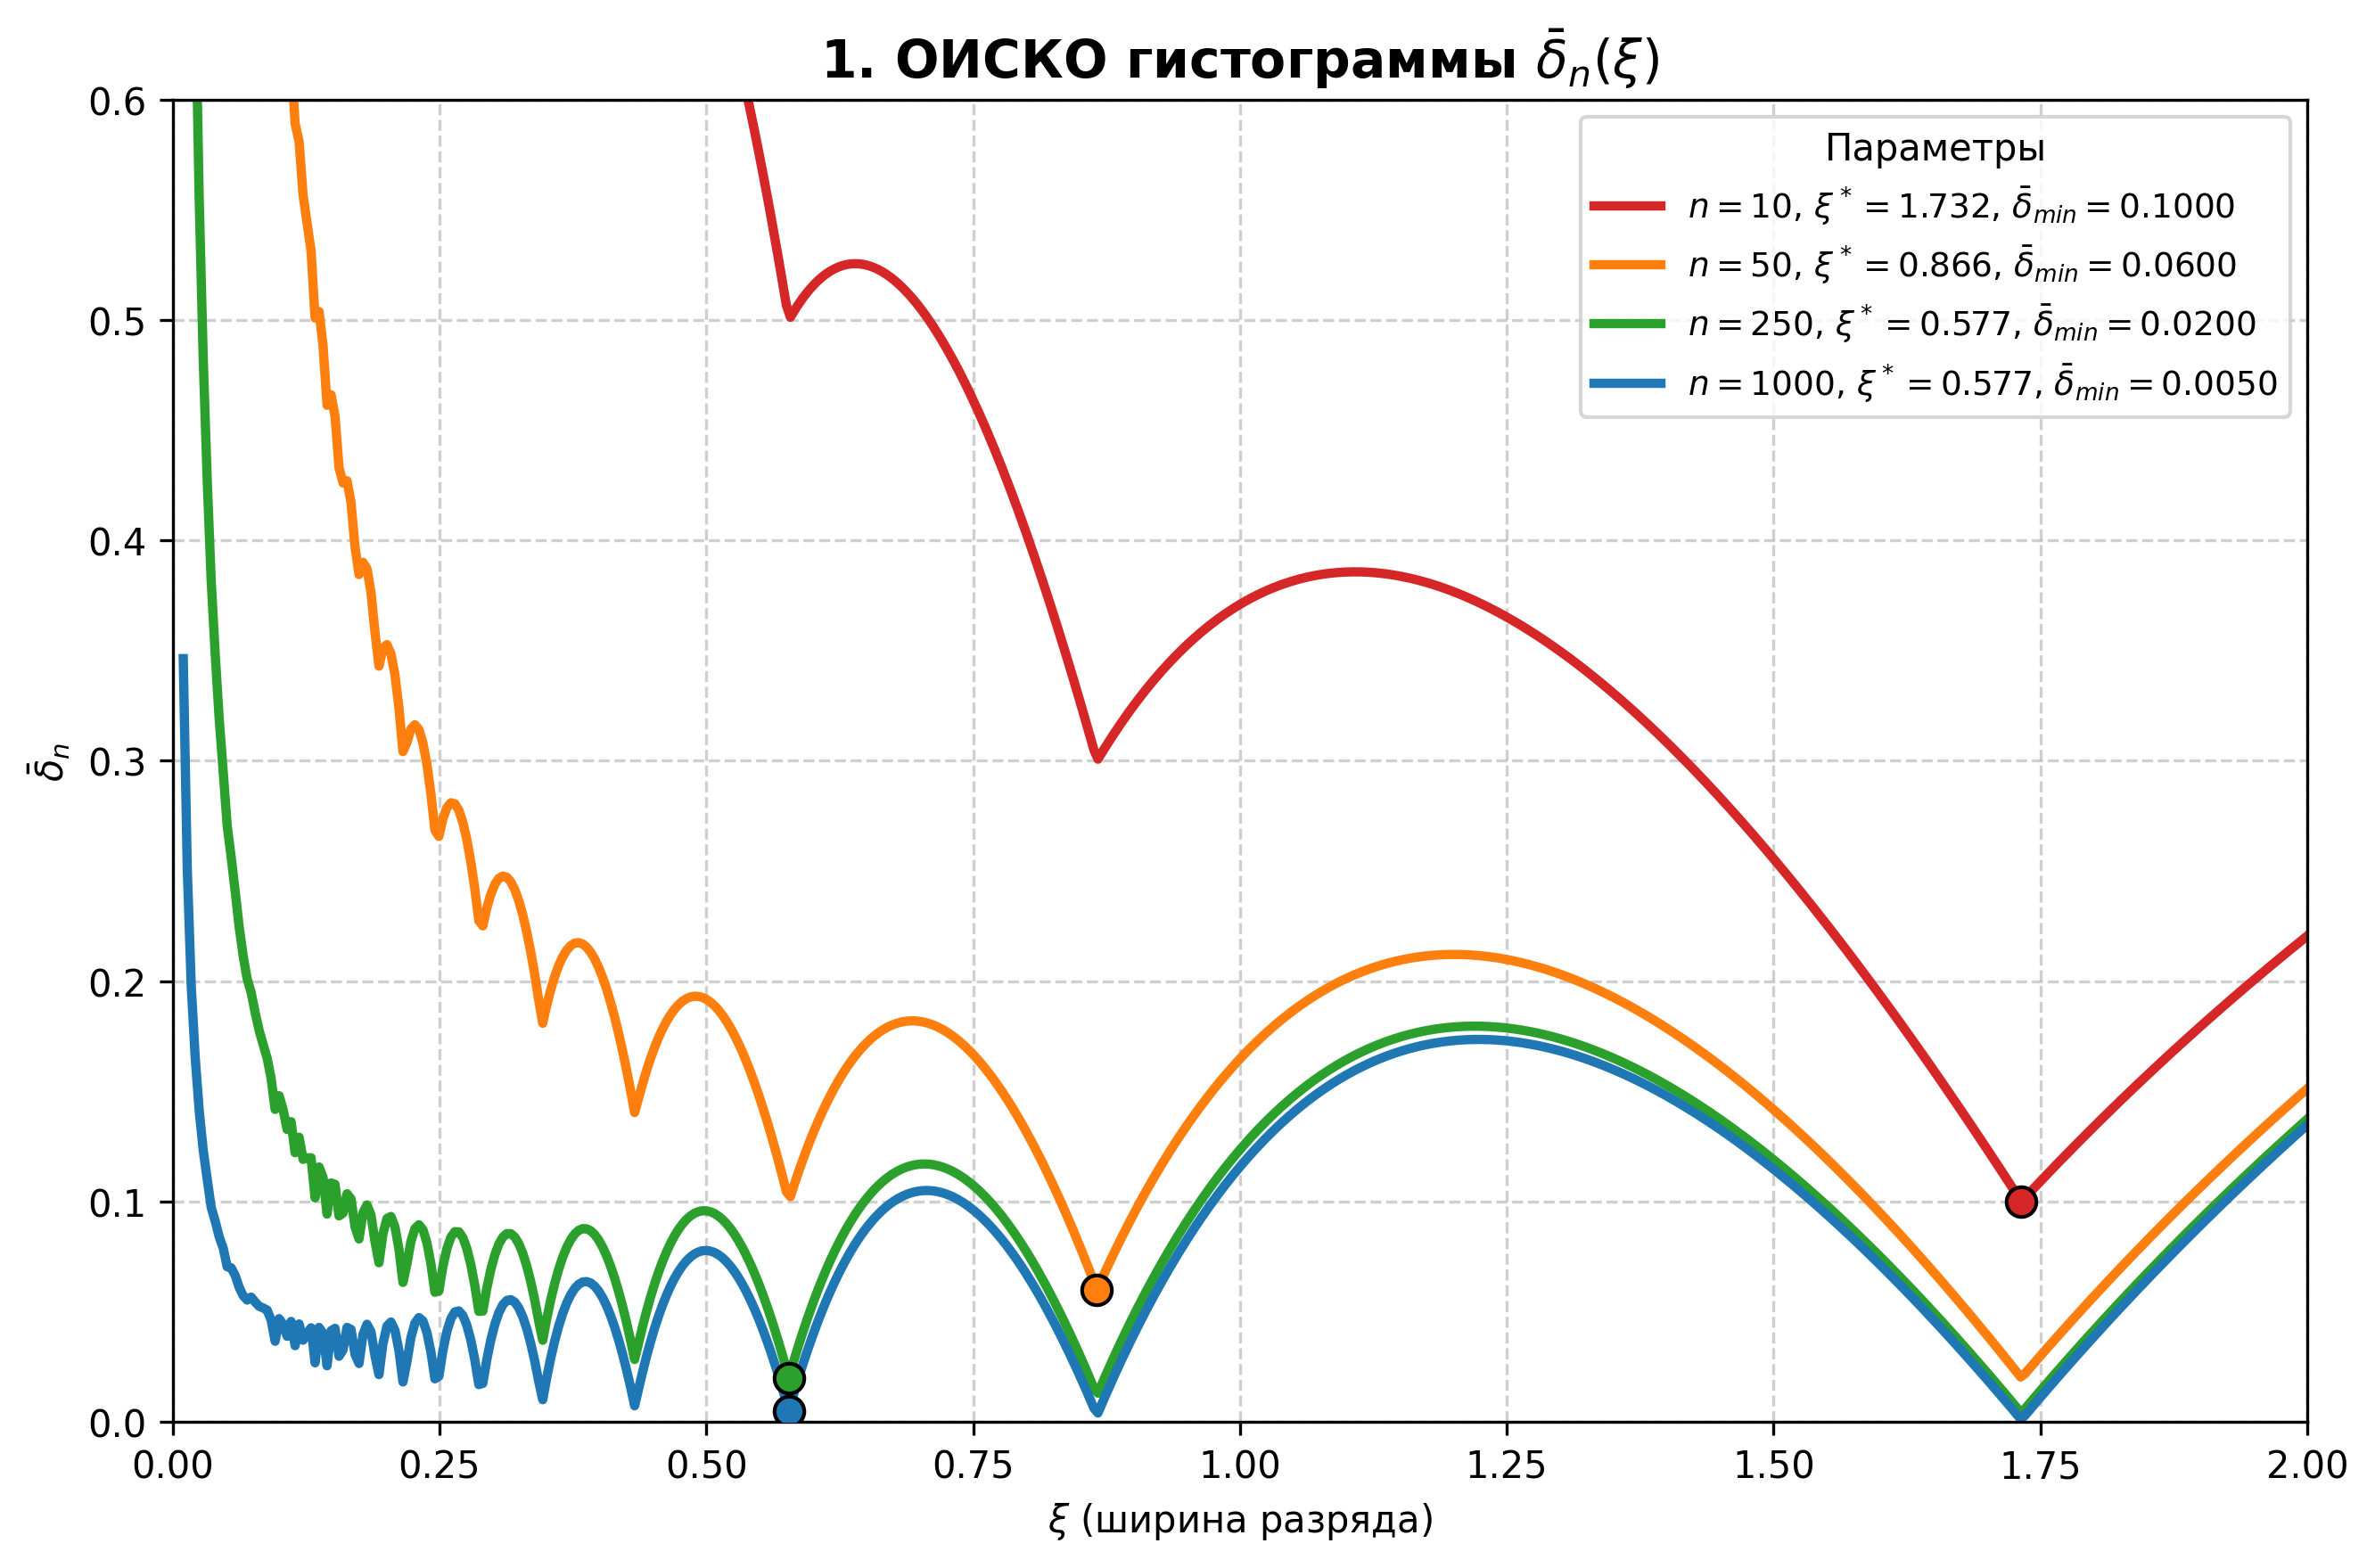
\includegraphics[width=0.85\textwidth]{figures/f5.png}
    \caption{ОИСКО гистограммы $\bar{\delta}_n(\xi)$ для $n = 10, 50, 250, 1000$}
    \label{fig:hist_delta_xi}
\end{figure}

\subsection*{График 2. Зависимость оптимального параметра $\xi_{opt}$ от $n$}

\begin{figure}[ht!]
    \centering
    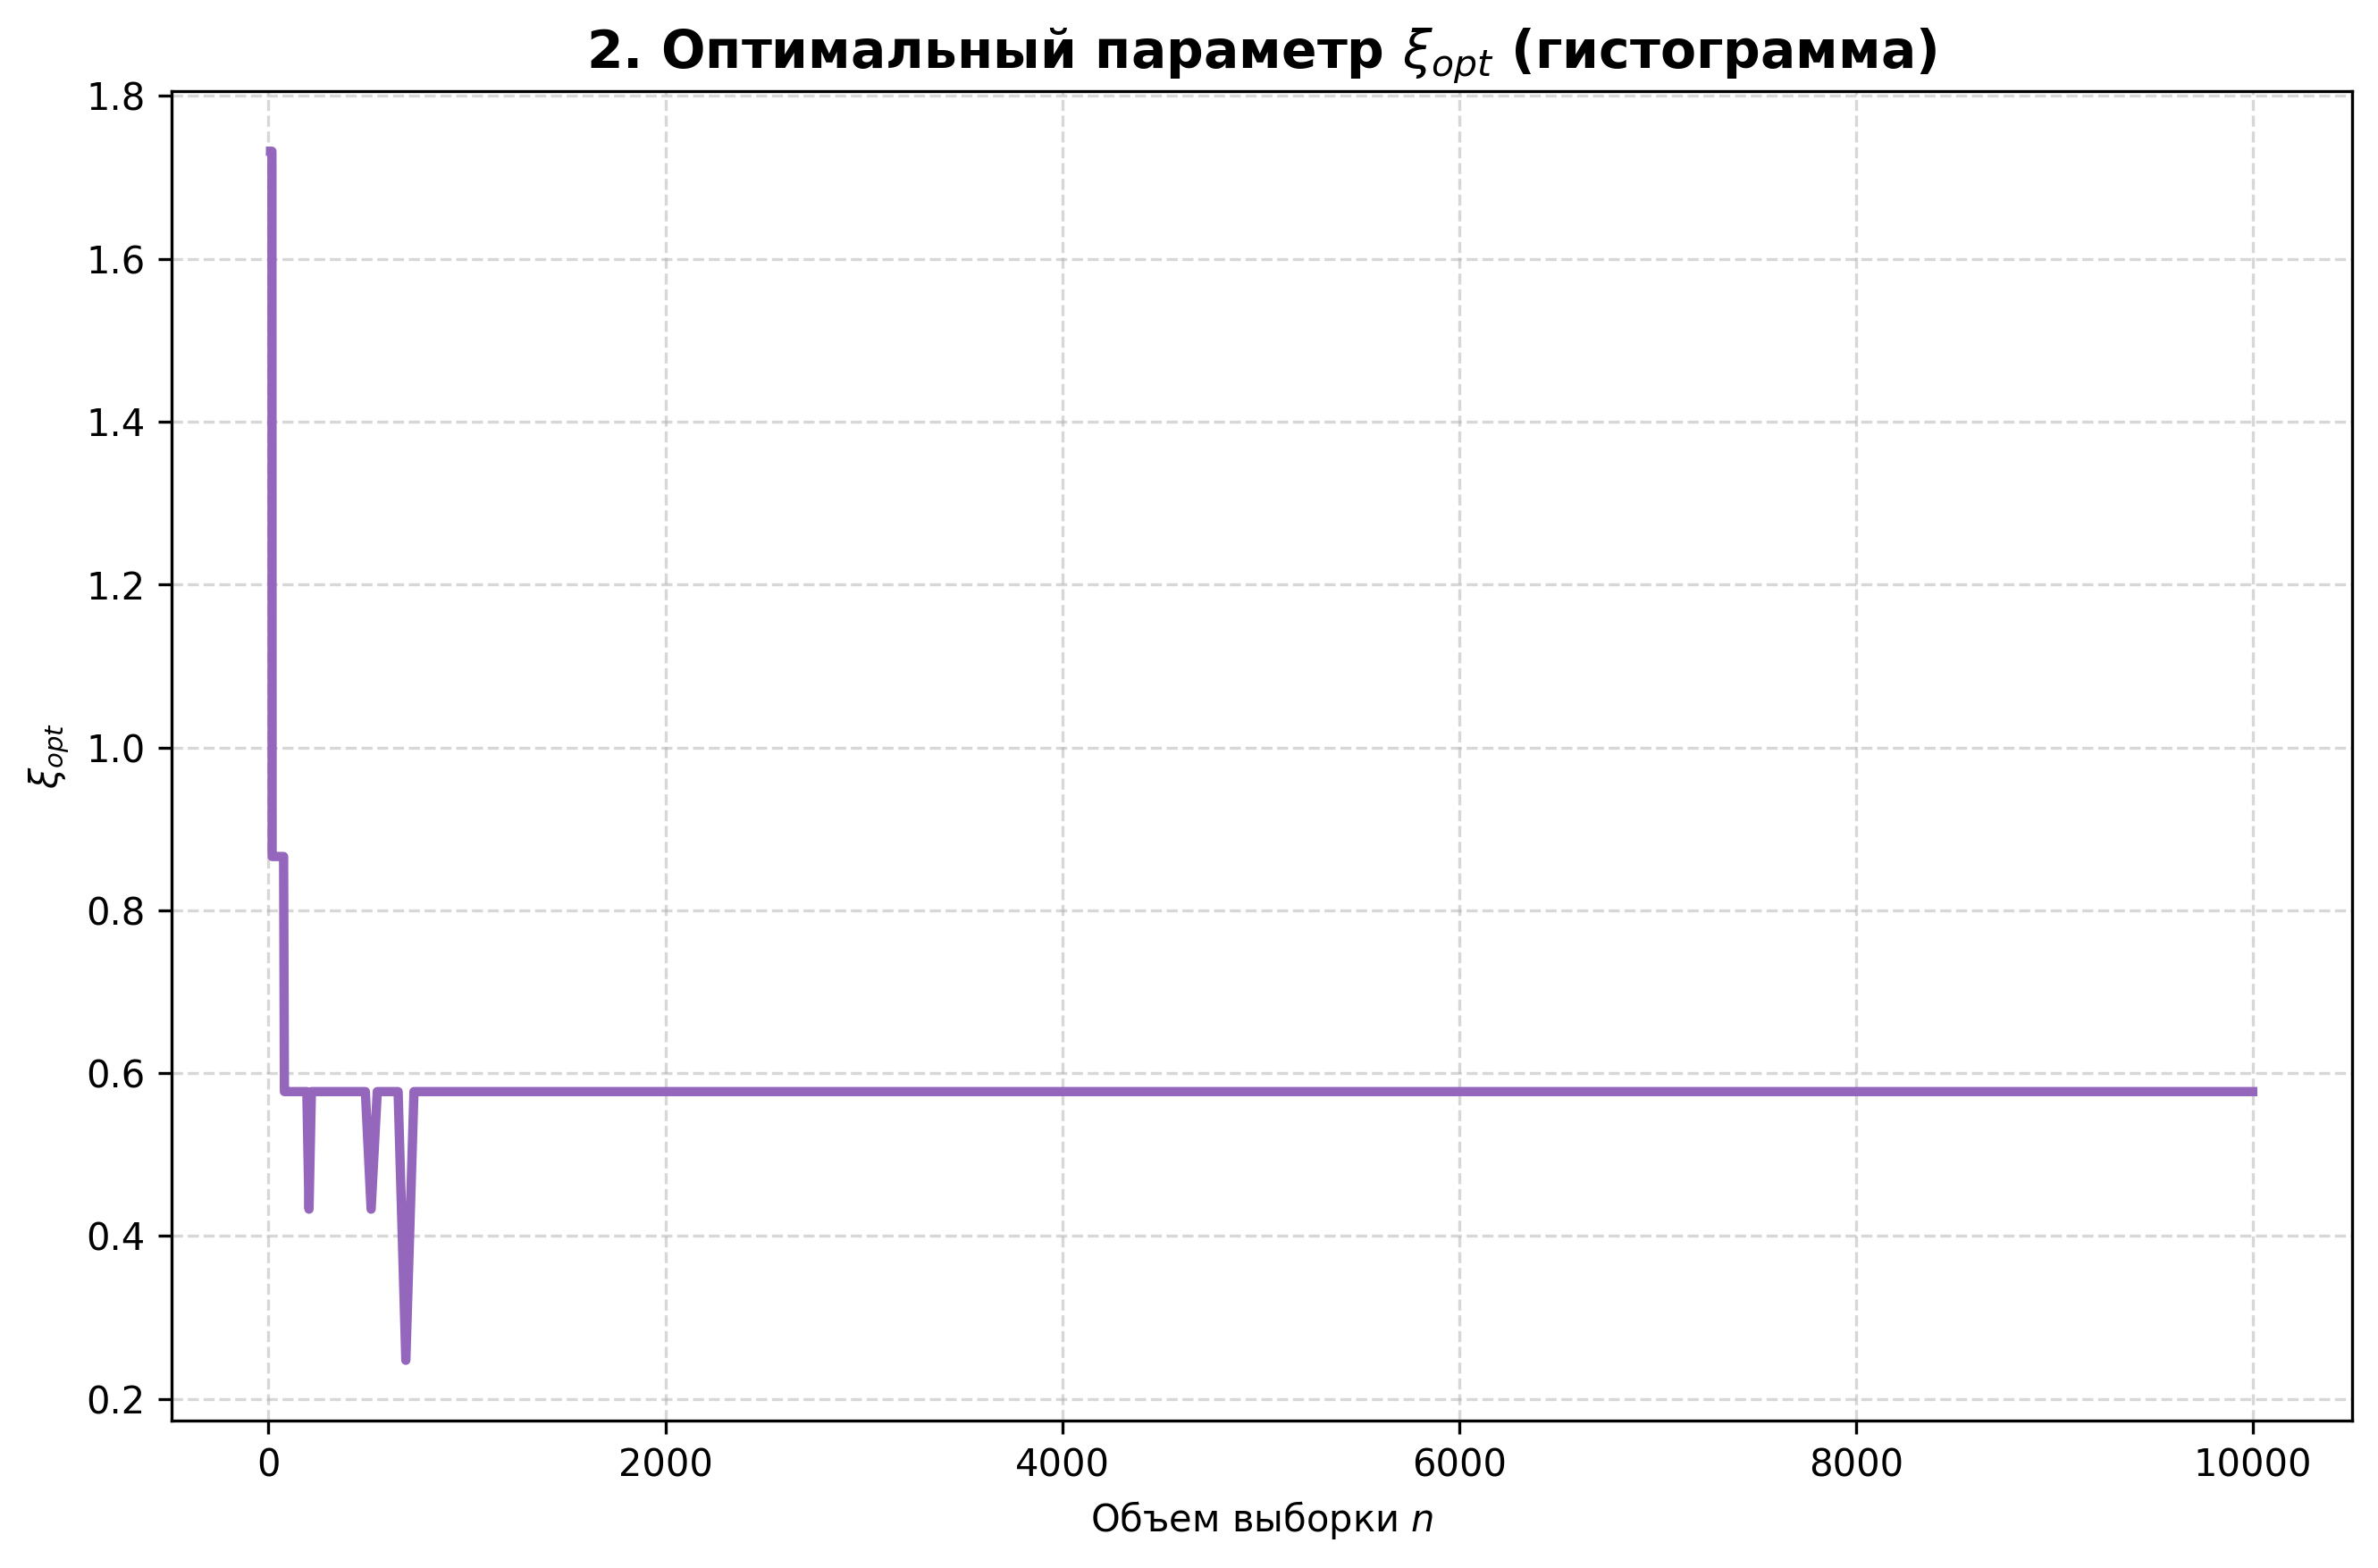
\includegraphics[width=0.85\textwidth]{figures/f6.png}
    \caption{Оптимальная ширина разряда $\xi_{opt}$ гистограммы в зависимости от объема выборки $n$}
    \label{fig:hist_xi_opt}
\end{figure}

\newpage
\subsection*{График 3. Зависимость нижней границы погрешности $\bar{\delta}_{n,\min}$ от $n$}

\begin{figure}[ht!]
    \centering
    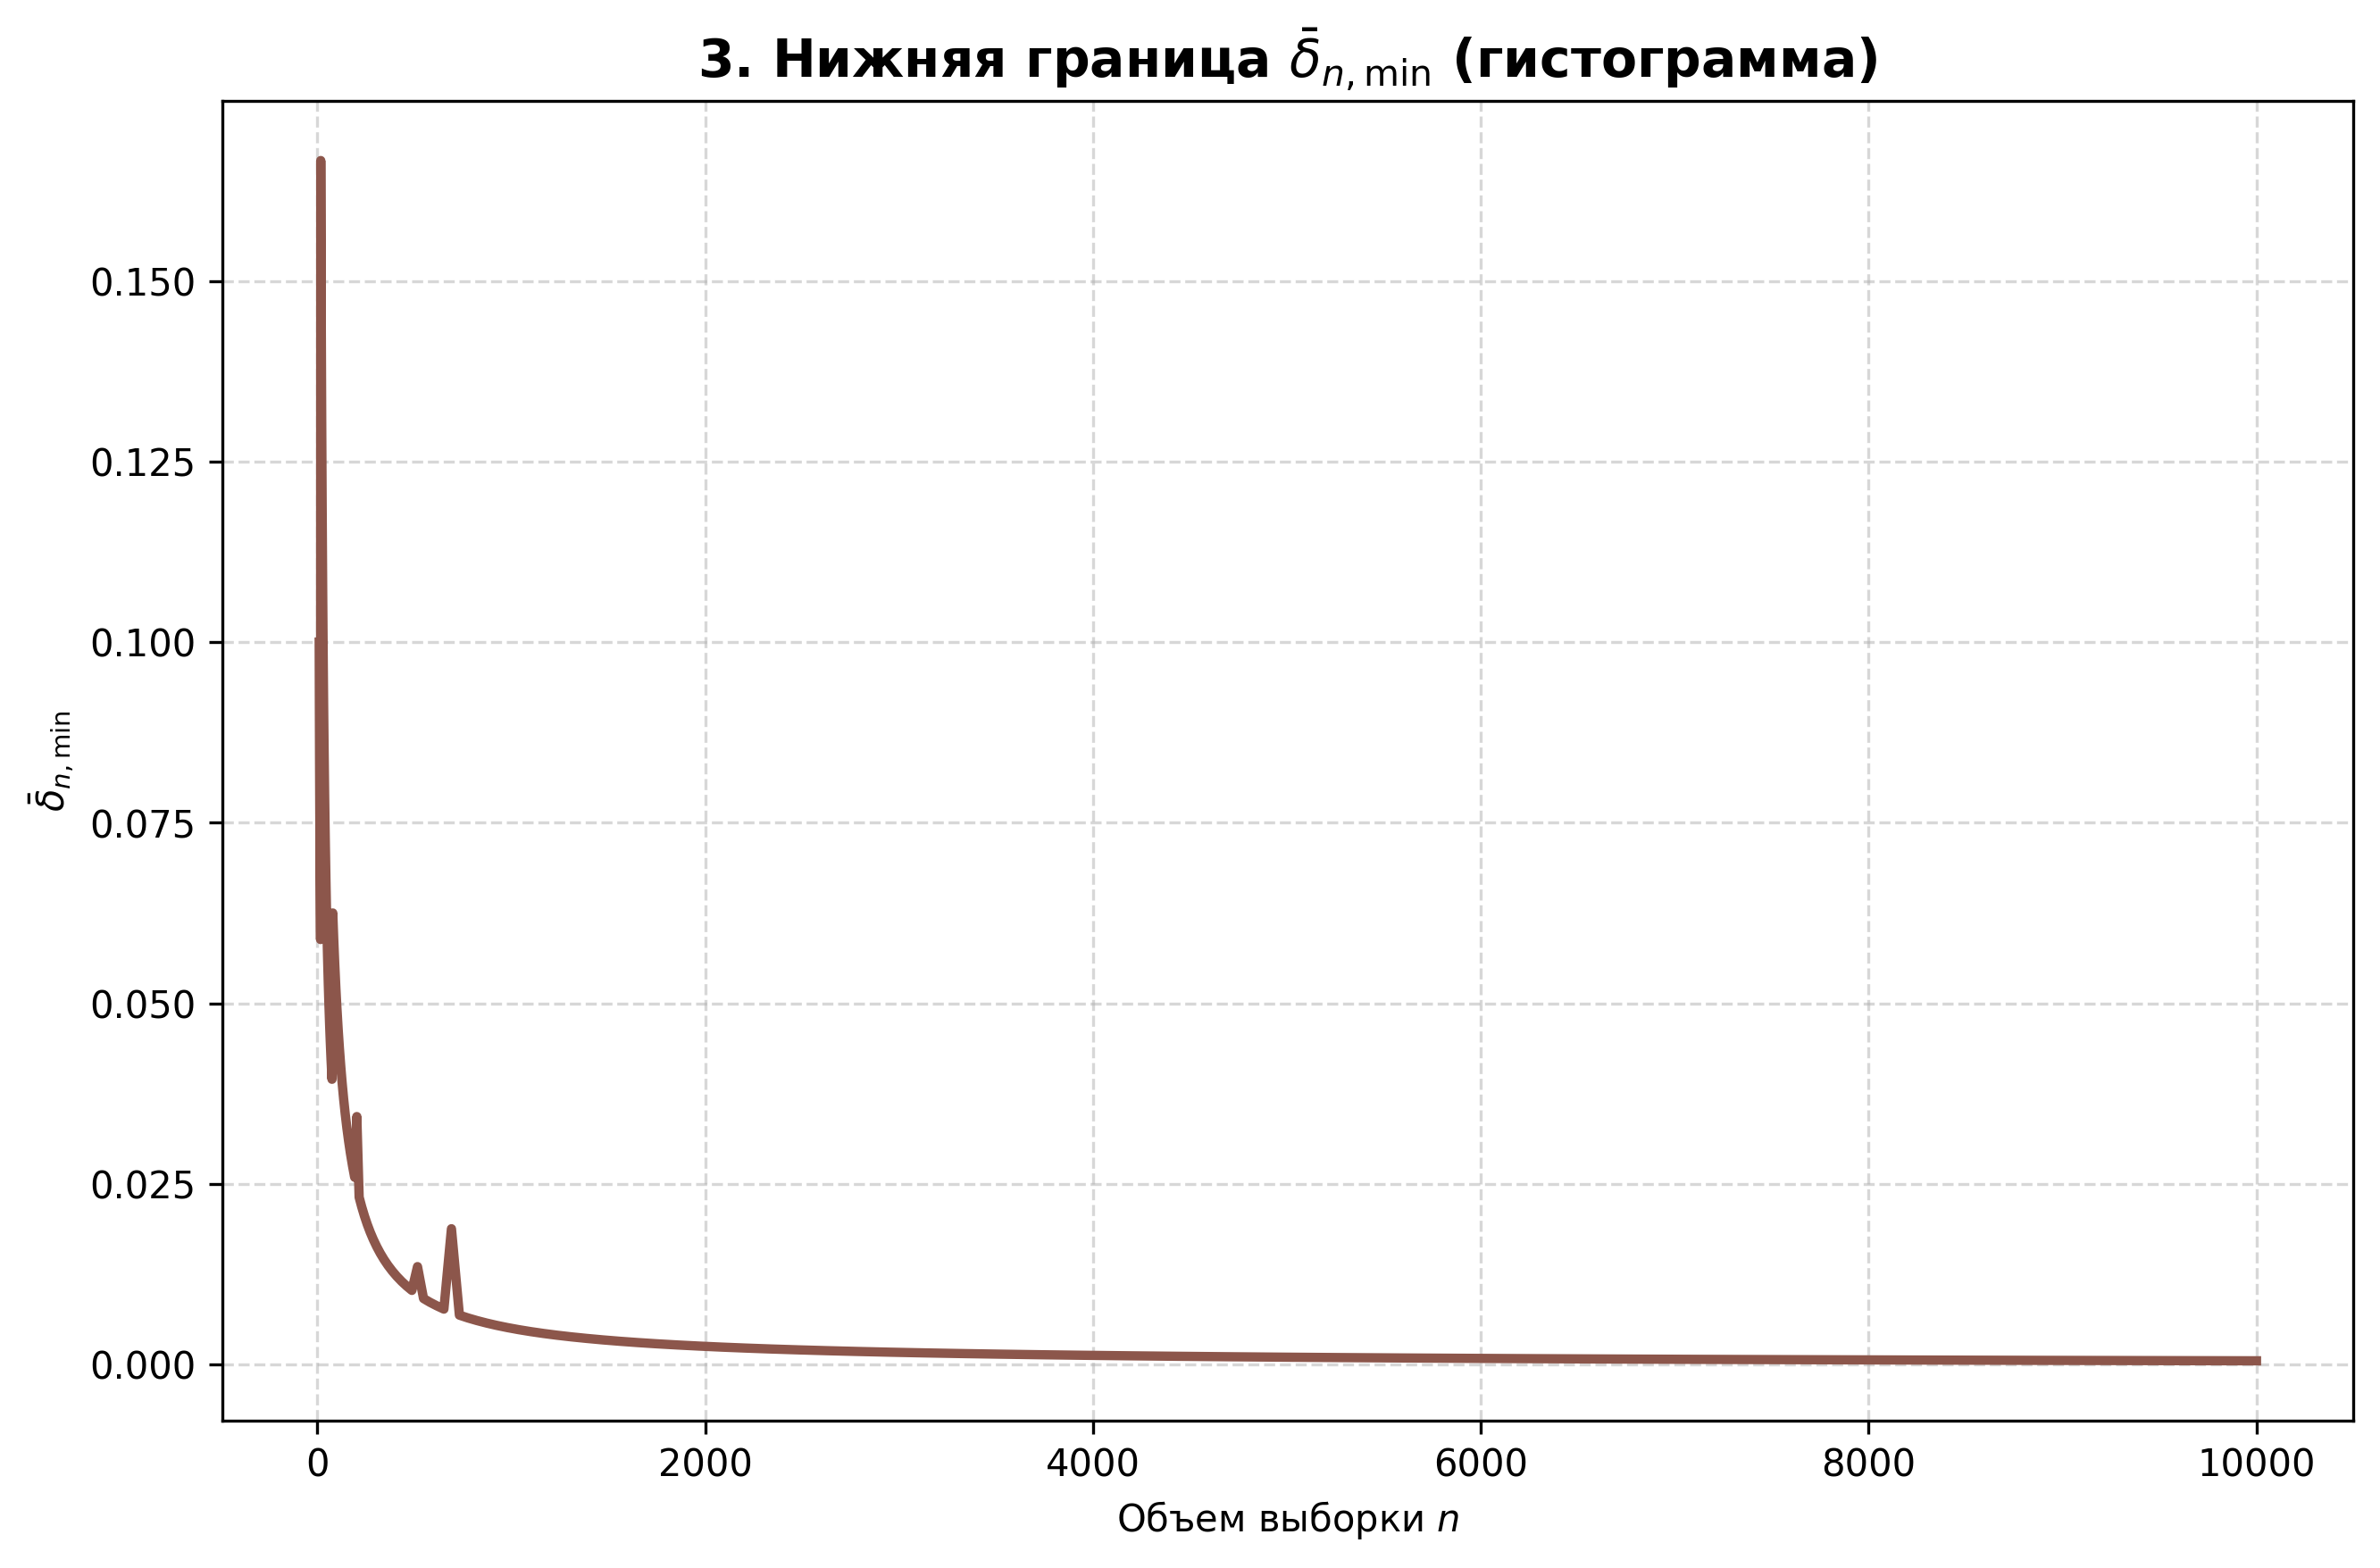
\includegraphics[width=0.85\textwidth]{figures/f7.png}
    \caption{Минимальное ОИСКО гистограммы $\bar{\delta}_{n,\min}(n)$}
    \label{fig:hist_delta_min}
\end{figure}

\subsection*{График 4. Сравнение ядерной оценки и гистограммы}

\begin{figure}[ht!]
    \centering
    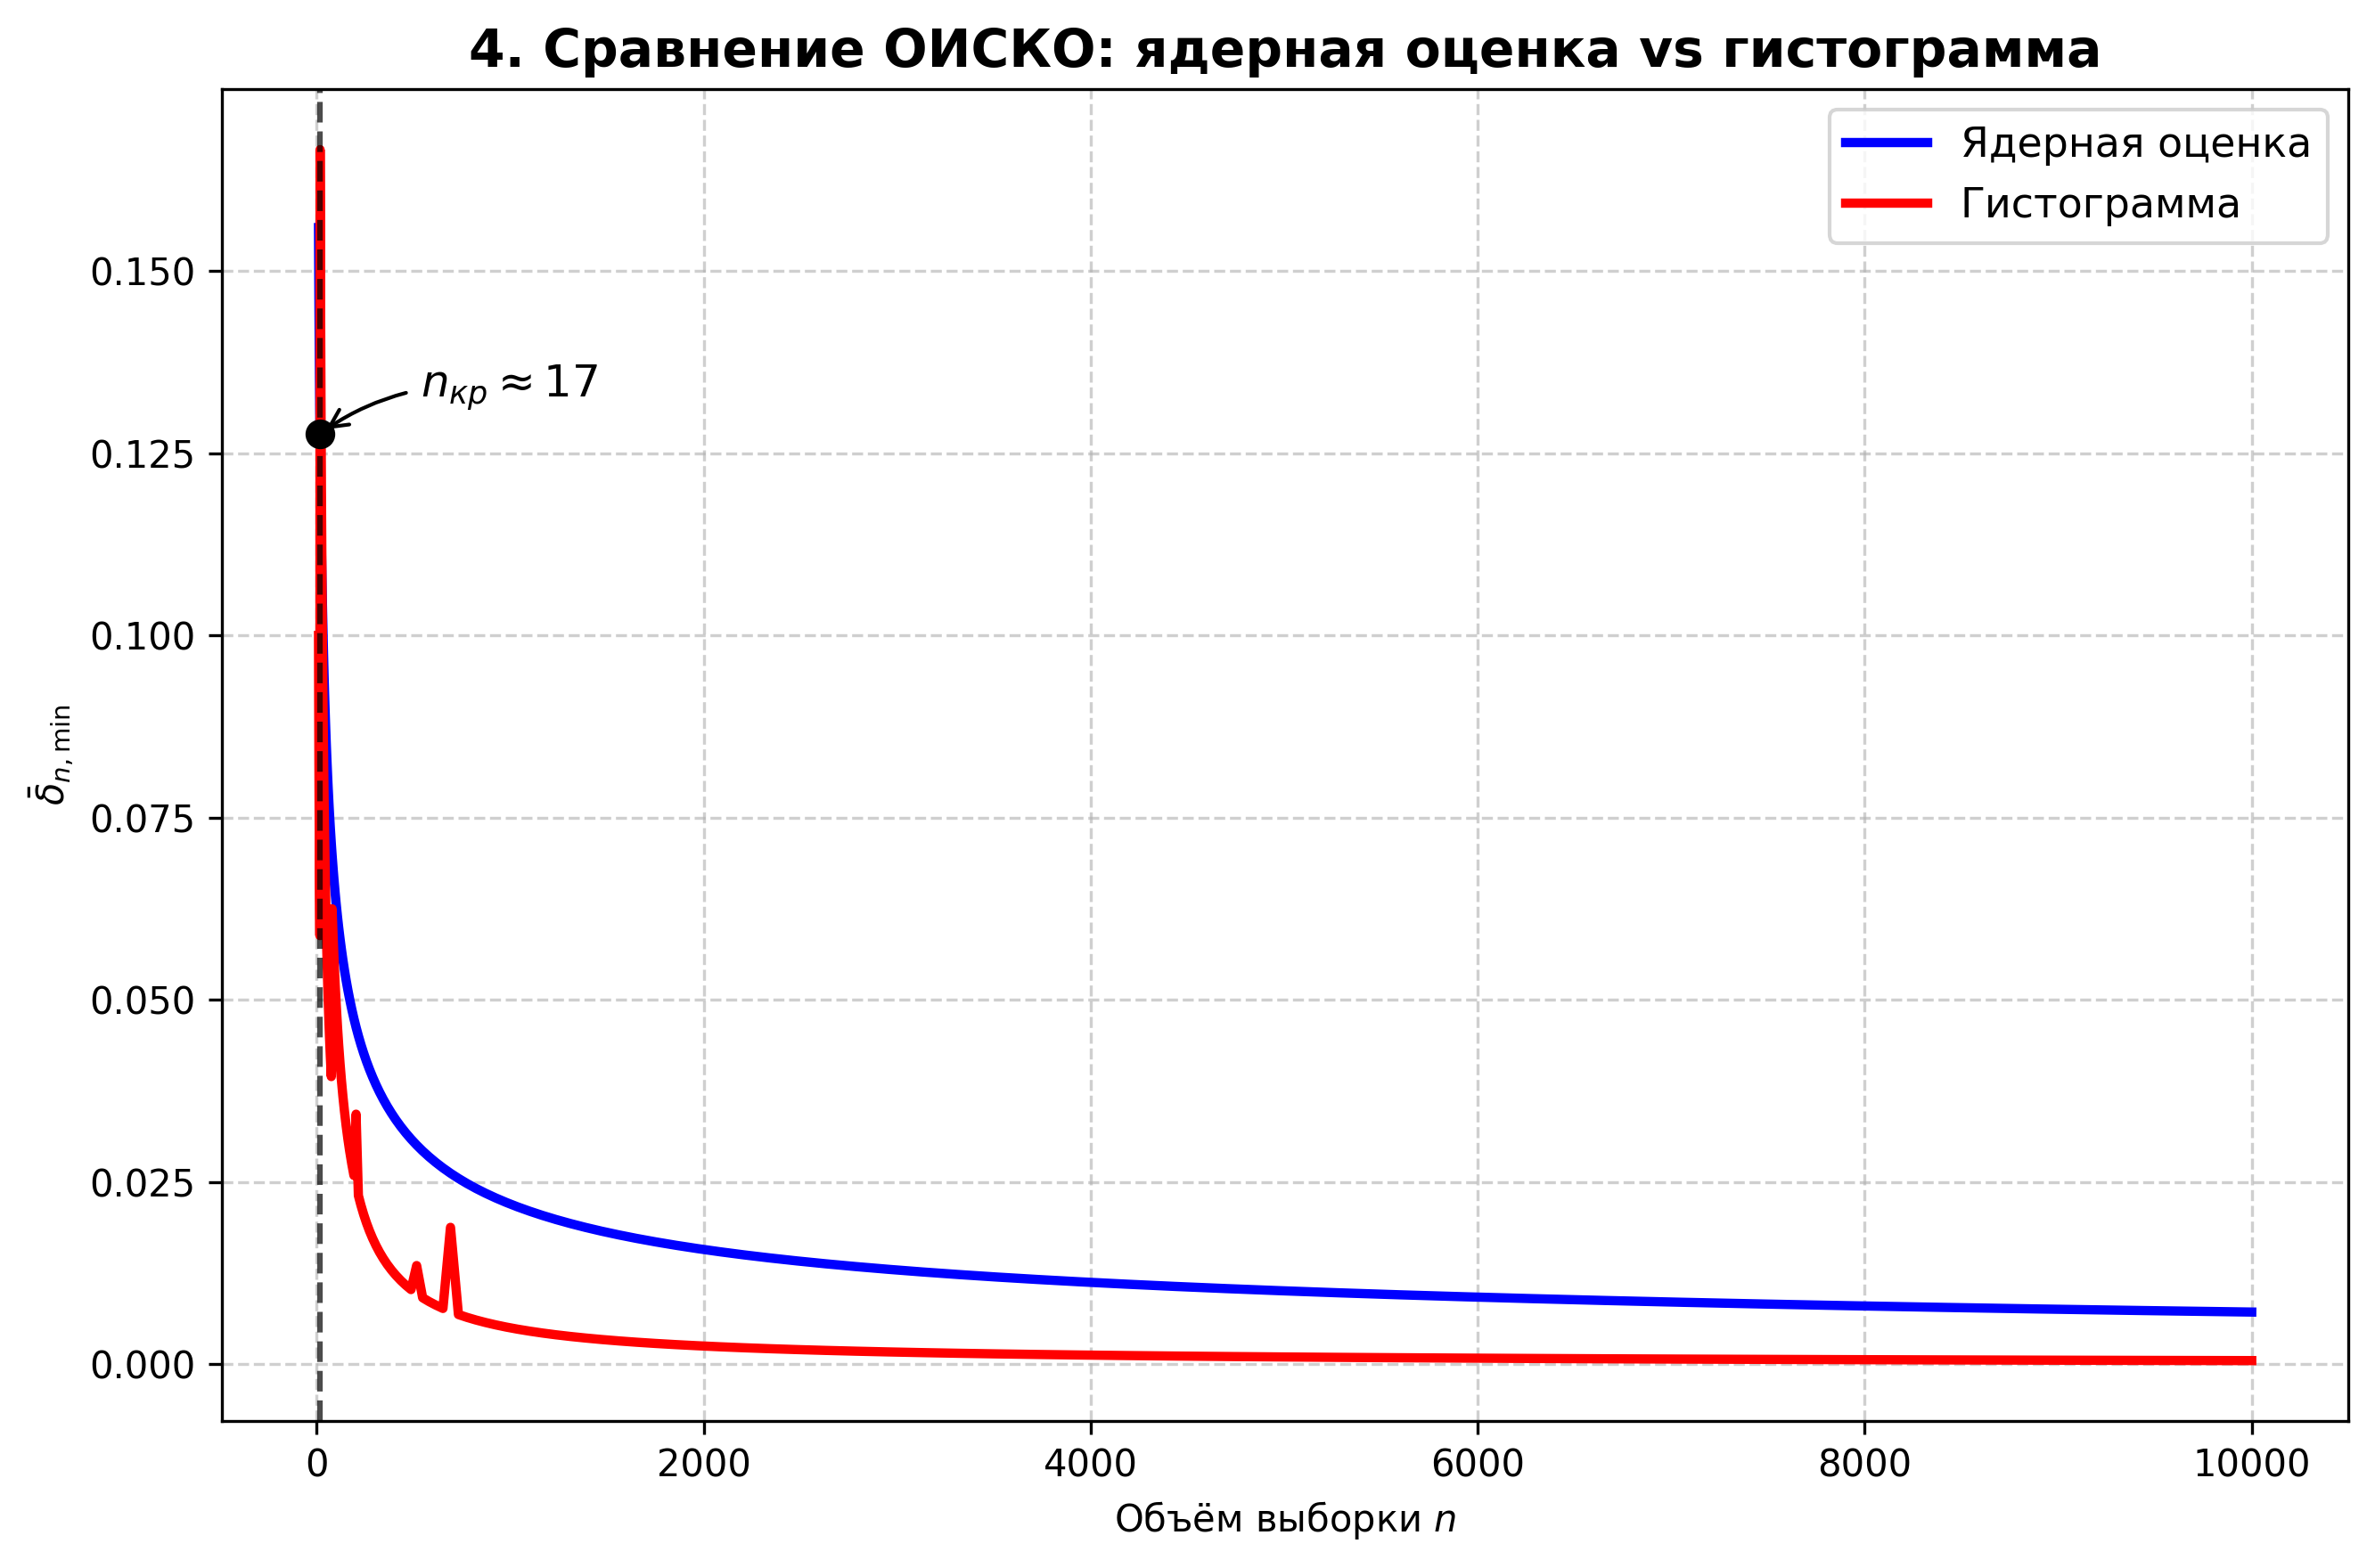
\includegraphics[width=0.85\textwidth]{figures/f8.png}
    \caption{Сравнение минимального ОИСКО ядерной оценки и гистограммы.}
    \label{fig:comparison}
\end{figure}

\end{document}